% 力矩

\pentry{矢量的叉乘\upref{Cross}}

\subsection{平面力矩}

如果只考虑一个厚度不计的片状物体在平面上的运动和受力, 受力点位矢为 $\bvec r$, 力为 $\bvec F$, 那么对于一个给定的参考点(除非明确指出, 一般取坐标原点), 就可以计算物体的受到的力矩.

\begin{figure}[ht]
\centering
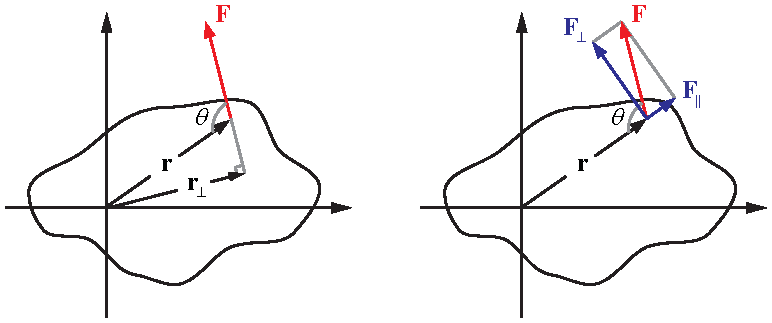
\includegraphics[width=13cm]{./figures/Torque1.pdf}
\caption{力矩的两种几何理解}\label{Torque_fig1}
\end{figure}

根据初中所学的方法,应该先作出“力臂” $\bvec r_ \bot$ 与力的方向垂直(\autoref{Torque_fig1} 左).力矩的大小(用 $\tau$ 表示)为
\begin{equation}\label{Torque_eq2}
\tau = \abs{\bvec r_ \bot } \abs{\bvec F} = \abs{\bvec r} \abs{\bvec F} \sin \theta 
\end{equation}
其中 $\theta $ 是 $\bvec r$ 与 $\bvec F$ 的夹角或其补角\footnote{因为 $\sin(\pi - \theta) = \sin\theta$}. 从另一种角度来看,也可以把力 $\bvec F$ 正交分解为平行
于 $\bvec r$ 的分量和垂直于 $\bvec r$ 的分量(\autoref{Torque_fig1} 右).其中平行分量不产
生力矩,垂直分量产生的力矩为
\begin{equation}\label{Torque_eq1}
\tau = \abs{\bvec r} \abs{\bvec F_ \bot } = \abs{\bvec r} \abs{\bvec F} \sin \theta 
\end{equation}
为了区分力矩的两个不同的方向(逆时针和顺时针),通常有两种做法:一是用正负号加以区分,例如规定逆时针的力矩为正,顺时针为负.这种定义把力矩看做一种标量(就像我们讨论一维运动时, 将速度表示成标量, 用正负号区分方向).另一种是根据叉乘的定义\upref{Cross}, 规定力矩为矢量,且
\begin{equation}\label{Torque_eq3}
\bvec \tau = \bvec r \cross \bvec F
\end{equation}
显然,由这种定义,力矩大小还是 $\tau = \abs{\bvec r} \abs{\bvec F}\sin \theta$, 但是逆时针力矩的方向垂直纸面指向读者,顺时针则相反.

\subsection{空间力矩}
若物体受到若干个力,且受力点不在一个平面内,或者力方向不在同一平面内,则应该在三维空间内考虑力矩,这时力矩只能是矢量,且仍然定义为\autoref{Torque_eq3}. 总力矩等于每个力所产生的力矩的矢量叠加.

\subsection{力矩的坐标系变换}
一般来说,由于受力点的位置矢量 $\bvec r$ 与坐标系的选取有关,现在来看力矩在不同坐标系之间的变换.

在坐标系 $A$ 中,第 $i$ 个受力点的位置矢量为 $\bvec r_{Ai}$, 物体的合力矩为
\begin{equation}
\bvec \tau_A = \sum_i \bvec r_{Ai} \cross \bvec F_i  = \bvec 0
\end{equation}
在另一坐标系 $B$ 中,$B$ 原点指向 $A$ 原点的矢量为 $\bvec r_{BA}$, 合力矩为
\begin{equation}\label{Torque_eq5}\ali{
\bvec \tau_B &= \sum_i (\bvec r_{Ai} + \bvec r_{BA}) \cross \bvec F_i = \sum_i \bvec r_{Ai} \cross \bvec F_i + \sum_i \bvec r_{BA} \cross \bvec F_i \\
&= \bvec \tau_A + \bvec r_{BA}\cross \sum_i \bvec F_i
}\end{equation}
其中最后两步使用了叉乘的分配律\upref{Cross}.由结论可以看出,变换坐标系,力矩需要加上原坐标系相对新坐标系的位移叉乘物体的合力.由此也可以得出,若物体的合力为零,则力矩与参考系无关.
